\documentclass{article}
\usepackage[backend=biber,natbib=true,style=alphabetic,maxbibnames=50]{biblatex}
\addbibresource{/home/nqbh/reference/bib.bib}
\usepackage[utf8]{vietnam}
\usepackage{tocloft}
\renewcommand{\cftsecleader}{\cftdotfill{\cftdotsep}}
\usepackage[colorlinks=true,linkcolor=blue,urlcolor=red,citecolor=magenta]{hyperref}
\usepackage{amsmath,amssymb,amsthm,float,graphicx,mathtools,tikz}
\usepackage{enumitem}
\setlist{leftmargin=4mm}
\usetikzlibrary{angles,calc,intersections,matrix,patterns,quotes,shadings}
\allowdisplaybreaks
\newtheorem{assumption}{Assumption}
\newtheorem{baitoan}{}%{Bài toán}
\newtheorem{cauhoi}{Câu hỏi}
\newtheorem{conjecture}{Conjecture}
\newtheorem{corollary}{Corollary}
\newtheorem{dangtoan}{Dạng toán}
\newtheorem{definition}{Definition}
\newtheorem{dinhly}{Định lý}
\newtheorem{dinhnghia}{Định nghĩa}
\newtheorem{example}{Example}
\newtheorem{ghichu}{Ghi chú}
\newtheorem{hequa}{Hệ quả}
\newtheorem{hypothesis}{Hypothesis}
\newtheorem{lemma}{Lemma}
\newtheorem{luuy}{Lưu ý}
\newtheorem{nhanxet}{Nhận xét}
\newtheorem{notation}{Notation}
\newtheorem{note}{Note}
\newtheorem{principle}{Principle}
\newtheorem{problem}{Problem}
\newtheorem{proposition}{Proposition}
\newtheorem{question}{Question}
\newtheorem{remark}{Remark}
\newtheorem{theorem}{Theorem}
\newtheorem{vidu}{Ví dụ}
\usepackage[left=1cm,right=1cm,top=5mm,bottom=5mm,footskip=4mm]{geometry}
\def\labelitemii{$\circ$}
\DeclareRobustCommand{\divby}{%
	\mathrel{\vbox{\baselineskip.65ex\lineskiplimit0pt\hbox{.}\hbox{.}\hbox{.}}}%
}

\title{Problem: Root -- Bài Tập: Căn Thức}
\author{Nguyễn Quản Bá Hồng\footnote{Independent Researcher, Ben Tre City, Vietnam\\e-mail: \texttt{nguyenquanbahong@gmail.com}; website: \url{https://nqbh.github.io}.}}
\date{\today}

\begin{document}
\maketitle
\begin{abstract}
	Last updated version: \href{https://github.com/NQBH/elementary_STEM_beyond/blob/main/elementary_mathematics/grade_9/circle/problem/NQBH_circle_problem.pdf}{GitHub{\tt/}NQBH{\tt/}elementary STEM \& beyond{\tt/}elementary mathematics{\tt/}grade 9{\tt/}circle{\tt/}problem: set $\mathbb{Q}$ of circles [pdf]}.\footnote{\textsc{url}: \url{https://github.com/NQBH/elementary_STEM_beyond/blob/main/elementary_mathematics/grade_9/circle/problem/NQBH_circle_problem.pdf}.} [\href{https://github.com/NQBH/elementary_STEM_beyond/blob/main/elementary_mathematics/grade_9/circle/problem/NQBH_circle_problem.tex}{\TeX}]\footnote{\textsc{url}: \url{https://github.com/NQBH/elementary_STEM_beyond/blob/main/elementary_mathematics/grade_9/rational/problem/NQBH_circle_problem.tex}.}. 
\end{abstract}
\tableofcontents

%------------------------------------------------------------------------------%

\section{Bất Phương Trình}
Ta xét các dạng bất đẳng thức \& bất phương trình được sử dụng nhiều để tìm điều kiện xác định (ĐKXĐ) của căn thức bậc 2 \& tổng quát hơn là căn thức bậc chẵn (căn thức bậc lẻ luôn xác định miễn là biểu thức dưới dấu căn có nghĩa, không nhất thiết phải không âm như căn bậc chẵn bắt buộc).

\subsection{Bất phương trình chứa ẩn trong dấu giá trị tuyệt đối}
Với $f:D\subset\mathbb{R}\to\mathbb{R}$, $x\mapsto f(x)$ là 1 hàm số biến $x$, có $\forall a\in\mathbb{R}$, $a > 0$:
\begin{equation*}
	\boxed{|f(x)| < a\Leftrightarrow -a < f(x) < a,\ |f(x)|\le a\Leftrightarrow -a\le f(x)\le a,\ |f(x)| > a\Leftrightarrow\left[\begin{split}
		f(x) &< -a,\\
		f(x) &> a,
	\end{split}\right.,\ |f(x)| > a\Leftrightarrow\left[\begin{split}
	f(x) &\le -a,\\
	f(x) &\ge a.
	\end{split}\right.}
\end{equation*}
Để giải bất phương trình tích, ta thường sử dụng:

\begin{dinhly}[Dấu của nhị thức bậc nhất $ax + b$]
	Nhị thức $ax + b$, $a,b\in\mathbb{R}$, $a\ne0$, cùng dấu với $a$ với mọi giá trị của $x$ lớn hơn nghiệm của nhị thức (i.e., $a(ax + b) > 0$, $\forall x > -\frac{b}{a}$), trái dấu với $a$ với mọi giá trị của $x$ nhỏ hơn nghiệm của nhị thức (i.e., $a(ax + b) < 0$, $\forall x < -\frac{b}{a}$).
\end{dinhly}

\begin{baitoan}[\cite{Binh_Toan_9_tap_1}, Ví dụ 1, p. 5]
	Giải bất phương trình bậc 2: (a) $x^2 - 4x - 5 < 0$. (b) $x^2 - 2x - 1 > 0$. (c) $2x^2 - 6x + 5 > 0$.
\end{baitoan}

\begin{baitoan}[\cite{Binh_Toan_9_tap_1}, 1., p. 6]
	Giải bất phương trình bậc 2: (a) $x^2 - 4x - 21 > 0$. (b) $x^2 - 4x + 1 < 0$. (c) $3x^2 - x + 1 > 0$. (d) $2x^2 - 5x + 4 < 0$.
\end{baitoan}

\begin{baitoan}[Giải bất phương trình bậc nhất tổng quát]
	Giải \& biện luận theo $a,b,c\in\mathbb{R}$, $a\ne0$, bất phương trình: (a) $ax + b > 0$. (b) $ax + b < 0$. (c) $ax + b\le0$. (d) $ax + b\ge0$.
\end{baitoan}

\begin{baitoan}[Giải bất phương trình bậc nhất chứa trị tuyệt đối dạng tổng quát]
	Giải \& biện luận theo $a,b,c\in\mathbb{R}$, $a\ne0$, bất phương trình: (a) $|ax + b| > c$. (b) $|ax + b| < c$. (c) $|ax + b|\le c$. (d) $|ax + b|\ge c$.
\end{baitoan}

\begin{baitoan}[Giải bất phương trình bậc 2 tổng quát]
	Giải \& biện luận theo $a,b,c,d\in\mathbb{R}$, $a\ne0$, bất phương trình: (a) $ax^2 + bx + c > 0$. (b) $ax^2 + bx + c < 0$. (c) $ax^2 + bx + c\le0$. (d) $ax^2 + bx + c\ge0$.
\end{baitoan}

\begin{baitoan}[Giải bất phương trình bậc 2 chứa trị tuyệt đối dạng tổng quát]
	Giải \& biện luận theo $a,b,c,d\in\mathbb{R}$, $a\ne0$, bất phương trình: (a) $|ax^2 + bx + c| > d$. (b) $|ax^2 + bx + c| < d$. (c) $|ax^2 + bx + c|\le d$. (d) $|ax^2 + bx + c|\ge d$.
\end{baitoan}

\begin{baitoan}[Giải bất phương trình dạng tích tổng quát]
	Giải \& biện luận theo $a,x_i\in\mathbb{R}$, $\forall i = 1,2,\ldots,n$, với $n\in\mathbb{N}$, $a\ne0$, bất phương trình: (a) {\rm Bất phương trình bậc nhất dạng tích tổng quát:} $a(x - x_0) > 0$, $a(x - x_0) < 0$, $a(x - x_0)\le0$, $a(x - x_0)\ge0$. (b) {\rm Bất phương trình bậc 2 dạng tích tổng quát:} Với $x_1\le x_2$, $a(x - x_1)(x - x_2) > 0$, $a(x - x_1)(x - x_2) < 0$, $a(x - x_1)(x - x_2)\le0$, $a(x - x_1)(x - x_2)\ge0$. (c) {\rm Bất phương trình bậc 3 dạng tích tổng quát:} Với $x_1\le x_2\le x_3$, $a(x - x_1)(x - x_2)(x - x_3) > 0$, $a(x - x_1)(x - x_2)(x - x_3) < 0$, $a(x - x_1)(x - x_2)(x - x_3)\le0$, $a(x - x_1)(x - x_2)(x - x_3)\ge0$. (d) {\rm Bất phương trình bậc 4 dạng tích tổng quát:} Với $x_1\le x_2\le x_3\le x_4$, $a(x - x_1)(x - x_2)(x - x_3)(x - x_4) > 0$, $a(x - x_1)(x - x_2)(x - x_3)(x - x_4) < 0$, $a(x - x_1)(x - x_2)(x - x_3)(x - x_4)\le0$, $a(x - x_1)(x - x_2)(x - x_3)(x - x_4)\ge0$. (e${}^\star$) {\rm Bất phương trình bậc $n\in\mathbb{N}^\star$ dạng tích tổng quát:} Với $x_1\le x_2\le\cdots\le x_{n-1}\le x_n$, $a\prod_{i=1}^n (x - x_i) > 0$, $a\prod_{i=1}^n (x - x_i) < 0$, $a\prod_{i=1}^n (x - x_i)\le0$, $a\prod_{i=1}^n (x - x_i)\ge0$, trong đó sử dụng ký hiệu tích $\prod_{i=1}^n (x - x_i) = (x - x_1)(x - x_2)\cdots(x - x_n)$.
\end{baitoan}

\begin{baitoan}[Programming: Solve general inequations of product-form]
	Viết chương trình {\sf Pascal, Python, C{\tt/}C++} để giải các bất phương trình $P(x) > 0$, $P(x) < 0$, $P(x)\le0$, $P(x)\ge0$, với $P(x)\coloneqq a\prod_{i=1}^n (x - x_i) = a(x - x_1)(x - x_2)\cdots(x - x_n)$, trong đó $n\in\mathbb{N}^\star$, $a\in\mathbb{R}$, $a\ne0$, $x_i\in\mathbb{R}$, $\forall i = 1,2,\ldots,n$.
	\begin{itemize}
		\item {\sf Input.} Dòng 1: Số bộ test. Dòng 2: $n\in\mathbb{N}$, $a\in\mathbb{R}^\star$. Dòng 3: $n$ số thực không nhất thiết phân biệt chưa được sắp xếp thứ tự: $x_1,x_2,\ldots,x_n$. 
		\item {\sf Output.} 4 tập nghiệm của 4 bất phương trình $P(x) > 0$, $P(x) < 0$, $P(x)\le0$, $P(x)\ge0$.
		\item {\sf Sample.}
		\begin{table}[H]
			\centering\tt
			\begin{tabular}{|l|l|}
				\hline
				\verb|polynomial_inequation.inp| & \verb|polynomial_inequation.out| \\
				\hline
				2 & P(x) > 0: x < 2 \\
				1 -1.5 & P(x) < 0: x > 2 \\
				2 & P(x) <= 0: x >= 2 \\
				2 100 & P(x) >= 0: x <= 2 \\
				3 -4 & \\
				& P(x) > 0: x < -4 or x > 3 \\
				& P(x) < 0: -4 < x < 3 \\
				& P(x) <= 0: -4 <= x <= 3 \\
				& P(x) >= 0: x <= -4 or x => 3 \\
				\hline
			\end{tabular}
		\end{table}
	\end{itemize}
\end{baitoan}

%------------------------------------------------------------------------------%

\section{Căn Bậc 2 \& Số Vô Tỷ}
Ở Toán 7 (xem, e.g., \cite[\S5, pp. 27--29]{SGK_Toan_7_Canh_Dieu_tap_1}), ta đã biết dạng biểu diễn thập phân của số hữu tỷ là hữu hạn hoặc vô hạn tuần hoàn, dạng biểu diễn thập phân của số vô tỷ là vô hạn không tuần hoàn. Số hữu tỷ $a\in\mathbb{Q}$ nào cũng viết được dưới dạng $a = \dfrac{m}{n}$ với $m\in\mathbb{Z}$, $n\in\mathbb{N}^\star$.

\begin{baitoan}[\cite{Binh_boi_duong_Toan_9_tap_1}, p. 30]
	Chứng minh $\sqrt{3} + \sqrt{5},2\sqrt{3} - 3\sqrt{5},\sqrt{2} + \sqrt{3} + \sqrt{5}$ là 3 số vô tỷ.
\end{baitoan}

\begin{baitoan}
	Chứng minh tổng, hiệu, tích, thương của 2 số hữu tỷ (số chia $\ne0$) là 1 số hữu tỷ.
\end{baitoan}

\begin{proof}[Chứng minh]
	Gọi 2 số hữu tỷ bất kỳ là $\dfrac{a}{b}$ \& $\dfrac{c}{d}$ với $a,b,c,d\in\mathbb{Z}$, $bd\ne0$. Tổng, hiệu, tích, thương của 2 số hữu tỷ (số chia $\ne0$) là 1 số hữu tỷ vì:
	\begin{align*}
		\frac{a}{b}\pm\frac{c}{d} = \frac{ad\pm bc}{bd},\ \frac{a}{b}\cdot\frac{c}{d} = \frac{ac}{bd},\ \forall a,b,c,d\in\mathbb{Z},\,bd\ne0; \frac{a}{b}:\frac{c}{d} = \frac{a}{b}\cdot\frac{d}{c} = \frac{ad}{bc},\ \forall a,b,c,d\in\mathbb{Z},\,bcd\ne0,
	\end{align*}
	trong đó điều kiện $bcd\ne0$ đã đảm bảo số chia khác 0.
\end{proof}

\begin{baitoan}[\cite{Binh_Toan_9_tap_1}, Ví dụ 2, p. 7]
	Chứng minh tổng \& hiệu của 1 số hữu tỷ với 1 số vô tỷ là 1 số vô tỷ.
\end{baitoan}

\begin{proof}[Giải]
	Chứng minh bằng phản chứng. Giả sử tồn tại 2 số $a\in\mathbb{Q}$ \& $b\in\mathbb{R}\backslash\mathbb{Q}$ sao cho $c = a + b\in\mathbb{Q}$. Ta có $b = c - a$, mà hiệu của 2 số hữu tỷ $c,a$ là 1 số hữu tỷ nên $b\in\mathbb{Q}$, mâu thuẫn với giả thiết, nên $c$ phải là số vô tỷ. Chứng minh tương tự cho hiệu.
\end{proof}

\begin{baitoan}
	(a) Chứng minh tích, \& thương của 1 số hữu tỷ khác $0$ với 1 số vô tỷ là 1 số vô tỷ.\footnote{Không cần yêu cầu số vô tỷ khác 0 vì 0 là số hữu tỷ nên hiển nhiên 1 số vô tỷ bất kỳ luôn khác 0.} (b) Chứng minh nếu tích hoặc thương của 1 số hữu tỷ với 1 số vô tỷ là 1 số hữu tỷ thì số hữu tỷ đó bằng $0$. 
\end{baitoan}

\begin{baitoan}
	Xét tính hữu tỷ, vô tỷ của 2 số $a,b\in\mathbb{R}$ thỏa mãn: (a) $a + b\in\mathbb{Q}$. (b) $a - b\in\mathbb{Q}$. (c) $ab\in\mathbb{Q}$. (d) $\dfrac{a}{b}\in\mathbb{Q}$. (e) $a^2 + b^2\in\mathbb{Q}$. (f) $a^2 - b^2\in\mathbb{Q}$. (g) $a^3 + b^3\in\mathbb{Q}$. (h) $a^3 - b^3\in\mathbb{Q}$. (i) $a^m + b^n\in\mathbb{Q}$ với $m,n\in\mathbb{N}^\star$. (j) $a^m - b^n\in\mathbb{Q}$ với $m,n\in\mathbb{N}^\star$.
\end{baitoan}

\begin{baitoan}[\cite{Binh_Toan_9_tap_1}, Ví dụ 3, p. 7]
	Xét xem 2 số $a,b$ có thể là số vô tỷ hay không, nếu: (a) $a + b$ \& $a - b$ là 2 số hữu tỷ. (b) $a - b$ \& $ab$ là 2 số hữu tỷ.
\end{baitoan}

\begin{baitoan}[\cite{Binh_Toan_9_tap_1}, Ví dụ 4, p. 7]
	Chứng minh: Nếu số tự nhiên $a$ không là số chính phương thì $\sqrt{a}$ là số vô tỷ.
\end{baitoan}

\begin{baitoan}[Mở rộng \cite{Binh_Toan_9_tap_1}, Ví dụ 4, p. 7]
	Chứng minh: Nếu số hữu tỷ $a$ không có dạng $\dfrac{m^2}{n^2}$ với $m,n\in\mathbb{N}$, $n\ne0$, thì $\sqrt{a}$ là số vô tỷ.
\end{baitoan}

\begin{baitoan}[\cite{Binh_Toan_9_tap_1}, 2., p. 8]
	Chứng minh các số sau là số vô tỷ: (a) $\sqrt{1 + \sqrt{2}}$. (b) $m + \dfrac{\sqrt{3}}{n}$ với $m,n\in\mathbb{Q}$, $n\ne0$.
\end{baitoan}

\begin{baitoan}[Mở rộng \cite{Binh_Toan_9_tap_1}, 2., p. 8]
	Cho $a,b,c\in\mathbb{Q}$. Tìm điều kiện của $a,b$ để: (a) $\sqrt{a + \sqrt{b}}\in\mathbb{Q}$. (b) $a + \dfrac{\sqrt{b}}{c}\in\mathbb{Q}$.
\end{baitoan}

\begin{baitoan}[\cite{Binh_Toan_9_tap_1}, 3., p. 8]
	Xét xem 2 số $a,b$ có thể là số vô tỷ hay không nếu: (a) $ab$ \& $\dfrac{a}{b}$ là các số hữu tỷ. (b) $a + b$ \& $\dfrac{a}{b}$ là các số hữu tỷ ($a + b\ne0$). (c) $a + b$, $a^2$, \& $b^2$ là các số hữu tỷ ($a + b\ne0$).
\end{baitoan}

\begin{baitoan}[\cite{Binh_Toan_9_tap_1}, 4., p. 8]
	So sánh 2 số: (a) $2\sqrt{3}$ \& $3\sqrt{2}$. (b) $6\sqrt{5}$ \& $5\sqrt{6}$. (c) $\sqrt{24} + \sqrt{45}$ \& $12$. (d) $\sqrt{37} - \sqrt{15}$ \& $2$.
\end{baitoan}

\begin{baitoan}[\cite{Binh_Toan_9_tap_1}, 5., p. 8]
	(a) Cho 1 ví dụ để chứng tỏ khẳng định $\sqrt{a}\le a$ với mọi số $a$ không âm là sai. (b) Cho $a > 0$. Với giá trị nào của $a$ thì $\sqrt{a} > a$?
\end{baitoan}

\begin{baitoan}[\cite{Binh_Toan_9_tap_1}, $\rm6^\star$., pp. 8--9]
	(a) Chỉ ra 1 số thực $x$ mà $x - \dfrac{1}{x}$ là số nguyên ($x\ne\pm1$). (b) Chứng minh nếu $x - \dfrac{1}{x}$ là số nguyên \& $x\ne\pm1$ thì $x$ \& $x + \dfrac{1}{x}$ là số vô tỷ. Khi đó $\left(x + \dfrac{1}{x}\right)^{2n}$ \& $\left(x + \dfrac{1}{x}\right)^{2n+1}$ là số hữu tỷ hay số vô tỷ?
\end{baitoan}

%------------------------------------------------------------------------------%

\section{Căn Thức Bậc 2 \& Hằng Đẳng Thức $\sqrt{A^2} = |A|$}

\begin{baitoan}[\cite{Binh_boi_duong_Toan_9_tap_1}, Ví dụ 1, p. 9]
	Trên 1 khúc sông, dòng chảy của nước ở bề mặt sông lớn hơn dòng chảy của nước ở đáy sông. Gọi $v$ {\rm km{\tt/}h} là vận tốc dòng chảy ở bề mặt sông, $f$ {\rm km{\tt/}h} là vận tốc dòng chảy ở đáy sông, các nhà vật lý (physicists) đã tính được $\sqrt{f} = \sqrt{v} - 1.3$. (a) Nếu vận tốc dòng chảy ở bề mặt sông là {\rm9 km{\tt/}h} thì vận tốc dòng chảy ở đáy sông là bao nhiêu? (b) Tính vận tốc dòng chảy ở bề mặt sông khi vận tốc dòng chảy ở đáy sông là {\rm20.25 km{\tt/}h}.
\end{baitoan}

\begin{baitoan}[\cite{Binh_boi_duong_Toan_9_tap_1}, Ví dụ 2, p. 9]
	Tìm $x\in\mathbb{R}$ thỏa: (a) $x^2 = 10$. (b) $\sqrt{2x + 1} = 5$. (c) $\sqrt{2x + 1} = \sqrt{3x - 1}$.
\end{baitoan}

\begin{baitoan}
	Giải \& biện luận phương trình theo các tham số $a,b,c,d\in\mathbb{R}$: (a) $x^2 = a$. (b) $\sqrt{ax + b} = c$. (c) $\sqrt{ax + b} = \sqrt{cx + d}$.
\end{baitoan}

\begin{baitoan}[\cite{Binh_boi_duong_Toan_9_tap_1}, Ví dụ 3, p. 10]
	So sánh: (a) $6$ \& $\sqrt{32}$. (b) $\sqrt{17} + \sqrt{10}$ \& $\sqrt{48}$. (c) $\sqrt{4 + \sqrt{5 + \sqrt{6}}}$ \& $3$.
\end{baitoan}

\begin{baitoan}[\cite{Binh_boi_duong_Toan_9_tap_1}, Ví dụ 4, p. 10]
	Rút gọn biểu thức: (a) $\sqrt{(a - 3)^2}$ với $a\le3$. (b) $2\sqrt{a^2 - 10a + 25}$ với $a\ge5$.
\end{baitoan}

\begin{baitoan}[\cite{Binh_boi_duong_Toan_9_tap_1}, Ví dụ 5, p. 10]
	Tìm $x\in\mathbb{R}$ thỏa: (a) $\sqrt{4x^2 - 28x + 49} = 7$. (b) $\sqrt{x - 10\sqrt{x} + 25} = 3$.
\end{baitoan}

\begin{baitoan}[\cite{Binh_boi_duong_Toan_9_tap_1}, Ví dụ 6, p. 11]
	Ngụy biện toán học: ``Bất kỳ 2 số nào cũng bằng nhau'': Với 2 số $a,b$ tùy ý, ta luôn có: $a^2 - 2ab + b^2 = b^2 - 2ba + a^2\Leftrightarrow(a - b)^2 = (b - a)^2$. Khai căn bậc 2 2 vế, ta được: $a - b = b - a$, suy ra $2a = 2b\Leftrightarrow a = b$. Vậy bất kỳ 2 số nào cũng bằng nhau. Tìm điểm sai.
\end{baitoan}

\begin{baitoan}[\cite{Binh_boi_duong_Toan_9_tap_1}, Ví dụ 7, p. 11]
	(a) Tìm {\rm GTNN} của biểu thức $A = \sqrt{x^2 - 8x + 20} - 12$. (b) Tìm {\rm GTLN} của biểu thức $B = 5 + \sqrt{-4x^2 - 4x + 6}$.
\end{baitoan}

\begin{luuy}
	(a) Để tìm {\rm GTNN} của 1 biểu thức $A$ có dạng $A = \sqrt{ax^2 + bx + c} + d$, ta cần biến đổi biểu thức dưới dấu căn của $A$ về dạng $f^2(x) + C$ ($C\ge0$ là hằng số) rồi nhận xét $\sqrt{f^2(x) + C}\ge\sqrt{C}$. Dấu ``$=$'' xảy ra $\Leftrightarrow f(x) = 0$. (b) Để tìm {\rm GTLN} của 1 biểu thức $B$ có dạng $B = \sqrt{ax^2 + bx + c} + d$, ta cần biến đổi biểu thức dưới dấu căn của $B$ về dạng $-f^2(x) + C$ ($C\ge0$  là hằng số) rồi nhận xét $\sqrt{-f^2(x) + C}\le\sqrt{C}$. Dấu ``$=$'' xảy ra $\Leftrightarrow f(x) = 0$.
\end{luuy}

\begin{baitoan}[\cite{Binh_boi_duong_Toan_9_tap_1}, 1.1., p. 12]
	Cho $\Delta ABC$ vuông tại $A$. Điền số thích hợp vào ô trống trong bảng:
	\begin{table}[H]
		\centering
		\begin{tabular}{|c|c|c|c|}
			\hline
			$AB$ & 7 cm & 0.3 m &  \\
			\hline
			$AC$ & 24 cm &  & 12 dm \\
			\hline
			$BC$ &  & 0.5 m & 15 dm \\
			\hline
		\end{tabular}
	\end{table}
\end{baitoan}

\begin{baitoan}[\cite{Binh_boi_duong_Toan_9_tap_1}, 1.2., p. 12]
	Tìm $x\in\mathbb{R}$ thỏa: (a) $3\sqrt{x + 1} = 18$. (b) $(2x)^2 = 64$. (c) $\sqrt{4x^2 - 4x + 1} = 7$.
\end{baitoan}

\begin{baitoan}[\cite{Binh_boi_duong_Toan_9_tap_1}, 1.3., p. 12]
	Tìm {\rm ĐKXĐ}: (a) $\sqrt{15 - 3x}$. (b) $\sqrt{\dfrac{x^2 + 1}{x - 1}}$. (c) $\sqrt{2x + 10} + \dfrac{1}{x^2 - 4}$.
\end{baitoan}

\begin{baitoan}[\cite{Binh_boi_duong_Toan_9_tap_1}, 1.4., p. 12]
	Tính: (a) $\sqrt{0.09}\cdot\sqrt{25} - \sqrt{49} + \sqrt{\dfrac{121}{100}}$. (b) $\sqrt{8^2 + 6^2} + 2\sqrt{\sqrt{625}}$.
\end{baitoan}

\begin{baitoan}[\cite{Binh_boi_duong_Toan_9_tap_1}, 1.5., p. 12]
	Cho 6 số: $\sqrt{21},5,\sqrt{38},-\sqrt{50},7,-\sqrt{37}$. Sắp xếp 6 số trên theo thứ tự tăng dần \& tìm số dương nhỏ nhất.
\end{baitoan}

\begin{baitoan}[\cite{Binh_boi_duong_Toan_9_tap_1}, 1.6., p. 12]
	Tính cạnh của hình vuông, biết diện tích của hình vuông đó bằng diện tích hình tam giác vuông có 2 cạnh góc vuông là {\rm12.8 m, 40 m}.
\end{baitoan}

\begin{baitoan}[\cite{Binh_boi_duong_Toan_9_tap_1}, 1.7., p. 12]
	Rút gọn biểu thức: (a) $\sqrt{(\sqrt{3} - 4)^2}$. (b) $\sqrt{6 - 2\sqrt{5}}$. (c) $\sqrt{4a^2} - 5a$ với $a > 0$. (d) $\sqrt{a^2 - 6a + 9} - 2\sqrt{a^2 + 8a + 16}$ với $-4\le a < 3$.
\end{baitoan}

\begin{baitoan}[\cite{Binh_boi_duong_Toan_9_tap_1}, 1.8., p. 12]
	Để tính giá trị của biểu thức $A = 3a + \sqrt{1 - 6a + 9a^2}$ tại $a = 2$, Việt làm như sau: $A = 3a + \sqrt{(1 - 3a)^2} = 3a + (1 - 3a) = 1$. Nam lại tính: $A = 3\cdot2 + \sqrt{1 - 6\cdot2 + 9\cdot2^2} = 6 + \sqrt{25} = 6 + 5 = 11$. Ai đúng ai sai? Sai ở đâu?
\end{baitoan}

\begin{baitoan}[\cite{Binh_boi_duong_Toan_9_tap_1}, 1.9., p. 12]
	Tìm $x\in\mathbb{R}$ thỏa: (a) $\sqrt{25x^2} = |-3|$. (b) $\sqrt{x^2 - 4x + 4} = \sqrt{x^2 + 4x + 4}$.
\end{baitoan}

\begin{baitoan}[\cite{Binh_boi_duong_Toan_9_tap_1}, 1.10., p. 12]
	Tìm {\rm GTLN} của biểu thức: (a) $A = \sqrt{7 - 2x^2}$. (b) $B = 7 + \sqrt{-4x^2 + 2x}$.
\end{baitoan}

\begin{baitoan}[\cite{Binh_boi_duong_Toan_9_tap_1}, 1.11., p. 13]
	Tìm {\rm GTNN} của biểu thức: (a) $A = 2\sqrt{x^2 + 3x + 5}$. (b) $B = \dfrac{3}{1 + \sqrt{2x - x^2 + 8}}$.
\end{baitoan}

\begin{baitoan}[\cite{Binh_boi_duong_Toan_9_tap_1}, 1.12., p. 13]
	Cho $a,b,c,d\in\mathbb{Q}$ thỏa $a + b + c + d = 0$. Chứng minh $\sqrt{(ab - cd)(bc - ad)(ca - bd)}\in\mathbb{Q}$.
\end{baitoan}

\begin{baitoan}[\cite{Binh_boi_duong_Toan_9_tap_1}, 1.13., p. 13]
	Cho hình vẽ:
	\begin{center}
		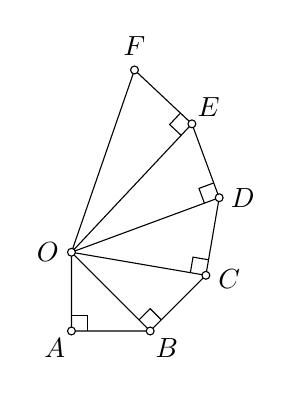
\begin{tikzpicture}
			\path
			(0,0) coordinate (A)
			(1,0) coordinate (B)
			(0,1) coordinate (O)
			($(B)!1cm!-90:(O)$) coordinate (C)
			($(C)!1cm!-90:(O)$) coordinate (D)
			($(D)!1cm!-90:(O)$) coordinate (E)
			($(E)!1cm!-90:(O)$) coordinate (F);
			\draw
			(O)--(A)--(B)--(C)--(D)--(E)--(F)--cycle (O)--(B) (O)--(C) (O)--(D) (O)--(E)
			pic[draw, angle radius=2mm]{right angle=O--A--B}
			pic[draw, angle radius=2mm]{right angle=O--B--C}
			pic[draw, angle radius=2mm]{right angle=O--C--D}
			pic[draw, angle radius=2mm]{right angle=O--D--E}
			pic[draw, angle radius=2mm]{right angle=O--E--F};
			\foreach \x/\g in {A/-135,B/-45,O/180,C/-10,D/0,E/45,F/90} \draw[fill=white] (\x) circle (.05) + (\g:.3) node{$\x$};
		\end{tikzpicture}
	\end{center}
	với $OA = AB = BC = CD = DE = EF = 1$ {\rm cm}. (a) Tính độ dài 5 đoạn t hẳng $OB,OC,OD,OE,OF$. (b) Vẽ đoạn thẳng có độ dài $\sqrt{10}$ {\rm cm}. (c) Nêu cách vẽ đoạn thẳng có độ dài $\sqrt{n}$ {\rm cm} với $n\in\mathbb{N}$ bằng thước thẳng \& compa.
\end{baitoan}

\begin{baitoan}[\cite{Binh_boi_duong_Toan_9_tap_1}, 1.14., p. 13]
	Tìm $n\in\mathbb{N}$ sao cho $\sqrt{4n + 1}\in\mathbb{N}$.
\end{baitoan}

\begin{baitoan}[\cite{Binh_boi_duong_Toan_9_tap_1}, 1.15., p. 13]
	Cho $A = \sqrt{2 + \sqrt{2 + \cdots + \sqrt{2}}}$ gồm $2015$ dấu căn bậc 2. Chứng minh $A\notin\mathbb{N}$.
\end{baitoan}

\begin{baitoan}[\cite{Binh_boi_duong_Toan_9_tap_1}, p. 14]
	Chứng minh đồng nhất thức: $\left(\dfrac{1}{a} + \dfrac{1}{b} + \dfrac{1}{c}\right)^2 = \dfrac{1}{a^2} + \dfrac{1}{b^2} + \dfrac{1}{c^2} + \dfrac{2(a + b + c)}{abc}$, $\forall a,b,c\in\mathbb{R}^\star$.
\end{baitoan}

\begin{baitoan}[\cite{Binh_boi_duong_Toan_9_tap_1}, p. 14]
	Chứng minh: $\sqrt{\dfrac{1}{a^2} + \dfrac{1}{b^2} + \dfrac{1}{c^2}} = \left|\dfrac{1}{a} + \dfrac{1}{b} + \dfrac{1}{c}\right|$, $\forall a,b,c\in\mathbb{R}^\star$ sao cho $a + b + c = 0$.
\end{baitoan}

\begin{baitoan}[\cite{Binh_boi_duong_Toan_9_tap_1}, p. 14]
	Chứng minh: $\sqrt{\dfrac{1}{a^2} + \dfrac{1}{b^2} + \dfrac{1}{(a + b)^2}} = \left|\dfrac{1}{a} + \dfrac{1}{b} - \dfrac{1}{a + b}\right|$, $\forall a,b\in\mathbb{R}^\star$, $a\ne-b$.
\end{baitoan}

\begin{baitoan}[\cite{Binh_boi_duong_Toan_9_tap_1}, p. 14]
	Chứng minh: $\sqrt{a^2 + \dfrac{1}{b^2} + \dfrac{a^2}{(ab + 1)^2}} = \left|a + \dfrac{1}{b} - \dfrac{a}{ab + 1}\right|$, $\forall a,b\in\mathbb{R}$, $b\ne0$, $ab\ne-1$.
\end{baitoan}

\begin{baitoan}[\cite{Binh_boi_duong_Toan_9_tap_1}, p. 14]
	Chứng minh: $\sqrt{a^2 + b^2 + \dfrac{a^2b^2}{(a + b)^2}} = \left|a + b - \dfrac{ab}{a + b}\right|$, $\forall a,b\in\mathbb{R}$, $a\ne-b$.
\end{baitoan}

\begin{baitoan}[\cite{Binh_boi_duong_Toan_9_tap_1}, 1., p. 14]
	Chứng minh với $a,b,c\in\mathbb{R}$ đôi một khác nhau: $\sqrt{\dfrac{1}{(a - b)^2} + \dfrac{1}{(b - c)^2} + \dfrac{1}{(c - a)^2}} = \left|\dfrac{1}{a - b} + \dfrac{1}{b - c} + \dfrac{1}{c - a}\right|$.
\end{baitoan}

\begin{baitoan}[\cite{Binh_boi_duong_Toan_9_tap_1}, 2., p. 15]
	Đơn giản biểu thức $A = \sqrt{\dfrac{1}{a^2 + b^2} + \dfrac{1}{(a + b)^2} + \sqrt{\dfrac{1}{a^4} + \dfrac{1}{b^4} + \dfrac{1}{(a^2 + b^2)^2}}}$, $\forall a,b\in\mathbb{R}^\star$, $a\ne-b$.
\end{baitoan}

\begin{baitoan}[\cite{Binh_boi_duong_Toan_9_tap_1}, 3., p. 15]
	Tính $A = \sqrt{1 + 2015^2 + \dfrac{2015^2}{2016^2}} + \dfrac{2015}{2016}$.
\end{baitoan}

\begin{baitoan}[\cite{Binh_boi_duong_Toan_9_tap_1}, 4., p. 15]
	Tính $A = \sqrt{0.43^2 + 0.57^2 + 0.43^2\cdot0.57^2}$.
\end{baitoan}

\begin{baitoan}
	Tính $A = \sqrt{x^2 + (1 - x)^2 + x^2\cdot(1 - x)^2}$, $\forall x\in\mathbb{R}$.
\end{baitoan}

\begin{baitoan}[\cite{Binh_boi_duong_Toan_9_tap_1}, p. 15]
	(a) Tính $A = \sum_{i=2}^{2015} \sqrt{1 + \dfrac{1}{i^2} + \dfrac{1}{(i + 1)^2}} = \sqrt{1 + \dfrac{1}{2^2} + \dfrac{1}{3^2}} + \sqrt{1 + \dfrac{1}{3^2} + \dfrac{1}{4^2}} + \cdots + \sqrt{1 + \dfrac{1}{2015^2} + \dfrac{1}{2016^2}}$. (b) Tính $A_n = \sum_{i=2}^n \sqrt{1 + \dfrac{1}{i^2} + \dfrac{1}{(i + 1)^2}} = \sqrt{1 + \dfrac{1}{2^2} + \dfrac{1}{3^2}} + \sqrt{1 + \dfrac{1}{3^2} + \dfrac{1}{4^2}} + \cdots + \sqrt{1 + \dfrac{1}{n^2} + \dfrac{1}{(n + 1)^2}}$, $\forall n\in\mathbb{N}^\star$.
\end{baitoan}

\begin{baitoan}[\cite{Binh_boi_duong_Toan_9_tap_1}, p. 15]
	(a) Tính $A = \sqrt{1 + \overline{\underbrace{99\ldots9}_{2015}}^2 + \overline{0.\underbrace{99\ldots9}_{2015}}^2}$. (b) Tính $A_n = \sqrt{1 + \overline{\underbrace{99\ldots9}_n}^2 + \overline{0.\underbrace{99\ldots9}_n}^2}$, $\forall n\in\mathbb{N}^\star$.
\end{baitoan}

%------------------------------------------------------------------------------%

\begin{baitoan}[\cite{Binh_Toan_9_tap_1}, Ví dụ 5, p. 7]
	Cho biểu thức $A = \sqrt{x - \sqrt{x^2 - 4x + 4}}$. (a) Tìm điều kiện xác định của biểu thức $A$. (b) Rút gọn biểu thức $A$.
\end{baitoan}

\begin{baitoan}[\cite{Binh_Toan_9_tap_1}, Ví dụ 6, p. 8]
	Tìm điều kiện xác định của các biểu thức: (a) $A = \dfrac{1}{\sqrt{x^2 - 2x - 1}}$. (b) $B = \dfrac{1}{\sqrt{x - \sqrt{2x + 1}}}$.
\end{baitoan}

\begin{baitoan}[\cite{Binh_Toan_9_tap_1}, Ví dụ 7, p. 8]
	Tìm các giá trị của $x$ sao cho $\sqrt{x + 1} < x + 3$.
\end{baitoan}

\begin{baitoan}[\cite{Binh_Toan_9_tap_1}, 7., p. 9]
	Tìm điều kiện xác định của các biểu thức: (a) $3 - \sqrt{1 - 16x^2}$. (b) $\dfrac{1}{1 - \sqrt{x^2 - 3}}$. (c) $\sqrt{8x - x^2 - 15}$. (d) $\dfrac{2}{\sqrt{x^2 - x + 1}}$. (e) $A = \dfrac{1}{\sqrt{x - \sqrt{2x - 1}}}$. (f) $B = \dfrac{\sqrt{16 - x^2}}{\sqrt{2x + 1}} + \sqrt{x^2 - 8x + 14}$.
\end{baitoan}

\begin{baitoan}[\cite{Binh_Toan_9_tap_1}, 8., p. 9]
	Cho biểu thức $A = \sqrt{x^2 - 6x + 9} - \sqrt{x^2 + 6x + 9}$. (a) Rút gọn biểu thức $A$. (b) Tìm các giá trị của $x$ để $A = 1$.
\end{baitoan}

\begin{baitoan}[\cite{Binh_Toan_9_tap_1}, 9., p. 9]
	Tìm các giá trị của $x$ sao cho: (a) $\sqrt{x^2 - 3}\le x^2 - 3$. (b) $\sqrt{x^2 - 6x + 9} > x - 6$.
\end{baitoan}

\begin{baitoan}[\cite{Binh_Toan_9_tap_1}, 10., p. 9]
	Cho $a + b + c = 0$ \& $abc\ne0$. Chứng minh hằng đẳng thức: $\sqrt{\dfrac{1}{a^2} + \dfrac{1}{b^2} + \dfrac{1}{c^2}} = \left|\dfrac{1}{a} + \dfrac{1}{b} + \dfrac{1}{c}\right|$.
\end{baitoan}

%------------------------------------------------------------------------------%

\section{Liên Hệ Giữa Phép Nhân, Phép Chia \& Phép Khai Phương}

\begin{baitoan}[\cite{Binh_boi_duong_Toan_9_tap_1}, p. 16]
	Với $A,B$ là 2 biểu thức đại số. Khi nào thì: $\sqrt{A + B} = \sqrt{A} + \sqrt{B}$. (b) $\sqrt{A - B} = \sqrt{A} - \sqrt{B}$?
\end{baitoan}

\begin{baitoan}[\cite{Binh_boi_duong_Toan_9_tap_1}, Ví dụ 1, p. 17]
	Tính: (a) $\sqrt{12.5\cdot10\cdot4500}$. (b) $\sqrt{685^2 - 684^2}$. (c) $\sqrt{\dfrac{27}{13}}:\sqrt{14\dfrac{10}{13}}$. (d) $\left(\sqrt{9 - \sqrt{17}} + \sqrt{9 + \sqrt{17}}\right)^2$.
\end{baitoan}

\begin{baitoan}[\cite{Binh_boi_duong_Toan_9_tap_1}, Ví dụ 2, p. 18]
	Tìm $x\in\mathbb{R}$ thỏa: (a) $\sqrt{8x}\cdot\sqrt{2} = 10$. (b) $\sqrt{x^2 - 9} - \sqrt{x + 3} = 0$. (c) $\dfrac{\sqrt{9x^2 - 25}}{\sqrt{3x - 5}} = 4$.
\end{baitoan}

\begin{baitoan}[\cite{Binh_boi_duong_Toan_9_tap_1}, Ví dụ 3, p. 18]
	2 bạn Việt \& Nam cùng giải bài toán tìm $x\in\mathbb{R}$: $\dfrac{\sqrt{2x - 5}}{\sqrt{x - 2}} = 2$. Việt làm như sau: $\dfrac{\sqrt{2x - 5}}{\sqrt{x - 2}} = 2\Leftrightarrow\sqrt{\dfrac{2x - 5}{x - 2}} = 2\Leftrightarrow\dfrac{2x - 5}{x - 2} = 4\Leftrightarrow2x - 5 = 4x - 8\Leftrightarrow2x = 3\Leftrightarrow x = 1.5$. Nam làm như sau: Điều kiện $2x - 5\ge0$ \& $x - 2> 0$, suy ra $x\ge2.5$. Rồi cũng giải để tìm ra $x = 1.5$ như Việt. Đối chiếu với điều kiện $x\ge2.5$, Nam kết luận phương trình vô nghiệm. Ai đúng ai sai? Giải thích.
\end{baitoan}

\begin{baitoan}[\cite{Binh_boi_duong_Toan_9_tap_1}, Ví dụ 4, p. 19]
	Rút gọn $(a + b)\sqrt{\dfrac{ab}{(a + b)^2}}$, $\forall a,b\in\mathbb{R}$, $a < 0$, $b < 0$.
\end{baitoan}

\begin{baitoan}[\cite{Binh_boi_duong_Toan_9_tap_1}, Ví dụ 5, p. 19]
	Rút gọn $A = \sqrt{2 + \sqrt{3}}\cdot \sqrt{2 + \sqrt{2 + \sqrt{3}}}\cdot\sqrt{2 + \sqrt{2 + \sqrt{2 + \sqrt{3}}}}\cdot\sqrt{2 - \sqrt{2 + \sqrt{2 + \sqrt{3}}}}$.
\end{baitoan}

\begin{baitoan}[\cite{Binh_boi_duong_Toan_9_tap_1}, Ví dụ 6, p. 19]
	Tính giá trị của biểu thức $A = \dfrac{x + 4 + 2\sqrt{16 - x^2}}{8 - 2x + \sqrt{16 - x^2}}$ tại $x = \dfrac{8}{\sqrt{3} + \frac{1}{\sqrt{3}}}$.
\end{baitoan}

\begin{baitoan}[\cite{Binh_boi_duong_Toan_9_tap_1}, Ví dụ 7, p. 20]
	(a) Cho $a\ge b\ge0$. Chứng minh: $\sqrt{a + b}\le\sqrt{a} + \sqrt{b}$, $\sqrt{a - b}\le\sqrt{a} - \sqrt{b}$. (b) Áp dụng: Tìm {\rm GTNN} của $A = \sqrt{x - 5} + \sqrt{7 - x}$ \& {\rm GTLN} của $B = \sqrt{2x - 7} - \sqrt{2x - 11}$.
\end{baitoan}

\begin{luuy}
	Khi chứng minh bất đẳng thức chứa căn thức ta thường bình phương 2 vế \& sử dụng tính chất: Với $A\ge0$, $B\ge0$, $A^2 > B^2\Rightarrow A > B$, $A^2\ge B^2\Rightarrow A\ge B$.
\end{luuy}

\begin{baitoan}[\cite{Binh_boi_duong_Toan_9_tap_1}, 2.1., p. 20]
	Tính đường kính của 1 mặt ghế hình tròn, biết diện tích của nó bằng diện tích hình vuông có cạnh là {\rm2.6 dm}.
\end{baitoan}

\begin{baitoan}[\cite{Binh_boi_duong_Toan_9_tap_1}, 2.2., p. 20]
	Rút gọn $\left(\sqrt{xy} - 2\sqrt{\dfrac{y}{x}}\right)\sqrt{xy}$, $\forall x,y\in\mathbb{R}$, $x < 0$, $y < 0$.
\end{baitoan}

\begin{baitoan}[\cite{Binh_boi_duong_Toan_9_tap_1}, 2.3., p. 20]
	Tìm $x\in\mathbb{R}$ thỏa $\sqrt{4x^2 - 25} = \sqrt{4x + 10}$.
\end{baitoan}

\begin{baitoan}[\cite{Binh_boi_duong_Toan_9_tap_1}, 2.4., p. 20]
	Tính: (a)$\left(\dfrac{1}{2}\sqrt{\dfrac{1}{2}}\right):\left(\dfrac{4}{15}\sqrt{\dfrac{1}{8}}\right)$. (b) $\sqrt{27(1 - \sqrt{3})^2}:3\sqrt{75}$.
\end{baitoan}

\begin{baitoan}[\cite{Binh_boi_duong_Toan_9_tap_1}, 2.5., p. 21]
	So sánh: (a) $x = \sqrt{16} + \sqrt{28}$, $y = \sqrt{14} + \sqrt{30}$. (b) $x = \dfrac{\sqrt{319^2 - 306^2}}{\sqrt{67^2 - 54^2}}$, $y = \sqrt{23 - 8\sqrt{7}}(4 + \sqrt{7}):(3\sqrt{3})$.
\end{baitoan}

\begin{baitoan}[\cite{Binh_boi_duong_Toan_9_tap_1}, 2.6., p. 21]
	Tính: $A = \sqrt{2 + \sqrt{2}}\cdot\sqrt{3 + \sqrt{7 + \sqrt{2}}}\cdot\sqrt{3 + \sqrt{6 + \sqrt{7 + \sqrt{2}}}}\cdot\sqrt{3 - \sqrt{6 + \sqrt{7 + \sqrt{2}}}}$.
\end{baitoan}

\begin{baitoan}[\cite{Binh_boi_duong_Toan_9_tap_1}, 2.7., p. 21]
	Cho 6 số thực dương $a_1,b_1,c_1,a_2,b_2,c_2$ thoả mãn điều kiện $\dfrac{a_1}{a_2} = \dfrac{b_1}{b_2} = \dfrac{c_1}{c_2}$. Chứng minh:
	\begin{align*}
		\sqrt{(a_1 + b_1 + c_1)(a_2 + b_2 + c_2)} = \sqrt{a_1a_2} + \sqrt{b_1b_2} + \sqrt{c_1c_2}.
	\end{align*}
\end{baitoan}

\begin{baitoan}[\cite{Binh_boi_duong_Toan_9_tap_1}, 2.8., p. 21]
	Tìm {\rm GTLN}: (a) $A = \sqrt{3x - 5} - \sqrt{3x - 10}$. (b) $B = \sqrt{4x + 1} - \sqrt{16x - 12}$.
\end{baitoan}

\begin{baitoan}[\cite{Binh_boi_duong_Toan_9_tap_1}, 2.9., p. 21]
	Chứng minh: nếu 3 đoạn thẳng có độ dài $a,b,c\in\mathbb{R}$ lập thành 1 tam giác thì 3 đoạn thẳng có độ dài $\sqrt{a},\sqrt{b},\sqrt{c}$ cũng lập thành 1 tam giác.
\end{baitoan}

\begin{baitoan}[\cite{Binh_boi_duong_Toan_9_tap_1}, 2.10., p. 21]
	Cho $x = \sqrt{4 + \sqrt{10 + 2\sqrt{5}}} + \sqrt{4 - \sqrt{10 + 2\sqrt{5}}}$. (a) Chứng minh $x^2 - 2x = 4$. (b) Tính giá trị của biểu thức $f(x) = \dfrac{x^4 - 4x^3 - x^2 + 10x + 4}{x^3 - 3x + 5}$.
\end{baitoan}

\begin{baitoan}[\cite{Binh_boi_duong_Toan_9_tap_1}, p. 21, Vận tốc của máy thăm dò vũ trụ]
	Vận tốc tối thiểu của máy thăm dò vũ trụ để thắng sức hút của Trái Đất là $v = 1.15\cdot10^{-5}\sqrt{\dfrac{m}{r}}$, trong đó $m$ là khối lượng của Trái Đất tính theo {\rm kg}, $r$ là bán kính Trái Đất tính theo {\rm m}, $v$ là vận tốc máy thăm dò tính theo {\rm m{\tt/}s}. Biết $m\approx5.98\cdot10^{24}$ {\rm kg}, $r\approx6.38\cdot10^6$ {\rm m}. Tính vận tốc tối thiểu của máy thăm dò vũ trụ.
\end{baitoan}

\begin{dinhnghia}[Trung bình cộng, trung bình nhân, trung bình điều hòa]
	Cho $a,b\in\mathbb{R}$, $a,b > 0$. $m\coloneqq\dfrac{a + b}{2}$ được gọi là {\rm trung bình cộng} của $a,b$. $n\coloneqq\sqrt{ab}$ được gọi là {\rm trung bình nhân} của $a,b$. $p\coloneqq\dfrac{2}{\frac{1}{a} + \frac{1}{b}}$ được gọi là {\rm trung bình điều hòa} của $a,b$.
\end{dinhnghia}

\begin{baitoan}[\cite{Binh_boi_duong_Toan_9_tap_1}, p. 22]
	Cho $a,b\in\mathbb{R}$, $a,b > 0$. Gọi $m,n,p$ lần lượt là trung bình cộng, trung bình nhân, trung bình điều hòa của $a,b$. Chứng minh $p\le n\le m$. Đẳng thức xảy ra khi nào?
\end{baitoan}

\begin{baitoan}[\cite{Binh_boi_duong_Toan_9_tap_1}, p. 22]
	Vẽ $\Delta ABC$ vuông tại $A$, đường cao $AH$, trung tuyến $AM$ sao cho $BH = a$, $CH = b$. Hạ $HD\bot AM$ tại $D$. Chứng minh $AD\le AH\le AO$. Từ đó suy ra bất đẳng thức $p\le n\le m$ với $m,n,p$ lần lượt là trung bình cộng, trung bình nhân, trung bình điều hòa của $a,b$.
	\begin{center}
		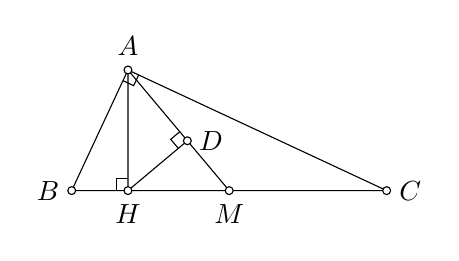
\begin{tikzpicture}
			\def\r{2}
			\path
			(130:\r) coordinate (A)
			(180:\r) coordinate (B)
			(0:\r) coordinate (C)
			($(B)!(A)!(C)$) coordinate (H)
			($(B)!.5!(C)$) coordinate (M)
			($(A)!(H)!(M)$) coordinate (D)
			;
			\draw
			(A)--(B)--(C)--cycle (A)--(H) (A)--(M) (H)--(D)
			pic[draw, angle radius=1.5mm]{right angle=B--A--C}
			pic[draw, angle radius=1.5mm]{right angle=A--H--B}
			pic[draw, angle radius=1.5mm]{right angle=A--D--H}			;
			\foreach \x/\g in {A/90,B/180,C/0,D/0,H/-90,M/-90} \draw[fill=white] (\x) circle (.05) + (\g:.3) node{$\x$};
		\end{tikzpicture}
	\end{center}
\end{baitoan}

\begin{dinhnghia}[Căn thức đồng dạng]
	2 căn thức bậc 2 được gọi là {\rm đồng dạng} nếu chúng có cùng biểu thức dưới dấu căn.
\end{dinhnghia}

\begin{vidu}[\cite{Binh_boi_duong_Toan_9_tap_1}, p. 22]
	(a) 3 biểu thức $\sqrt{7},2\sqrt{7},-5\sqrt{7}$ được gọi là {\rm đồng dạng} với nhau. (b) 3 biểu thức $\frac{1}{2}\sqrt{x},5\sqrt{x},-\frac{4}{7}\sqrt{x}$, $x\in\mathbb{R}$, $x\ge0$, được gọi là {\rm đồng dạng} với nhau.
\end{vidu}
Muốn cộng trừ các căn thức bậc 2 ta thu gọn các căn thức đồng dạng.

\begin{baitoan}[\cite{Binh_boi_duong_Toan_9_tap_1}, p. 23, Công thức căn phức tạp]
	Chứng minh:
	\begin{align}
		\label{can phuc tap}
		\sqrt{a\pm\sqrt{b}} = \sqrt{\frac{a + \sqrt{a^2 - b}}{2}}\pm\sqrt{\frac{a - \sqrt{a^2 - b}}{2}},\ \forall a,b\in\mathbb{R},\,a,b > 0,\,a^2\ge b.
	\end{align}
\end{baitoan}
Công thức \eqref{can phuc tap} được gọi là \textit{công thức căn phức tạp}. Nhờ công thức này, biểu thức $a\pm\sqrt{b}$ có thể dễ dàng viết được thành bình phương của 1 tổng hoặc hiệu, do đó tính được $a\pm\sqrt{b}$.

\begin{baitoan}[\cite{Binh_boi_duong_Toan_9_tap_1}, p. 23]
	Tính: (a) $A = 2\sqrt{3 + \sqrt{5 - \sqrt{13 + \sqrt{48}}}}$. (b) $B = \sqrt{4 + \sqrt{5\sqrt{3} + 5\sqrt{48 - 10\sqrt{7 + 4\sqrt{2}}}}}$.
\end{baitoan}

%------------------------------------------------------------------------------%

\section{Biến Đổi Đơn Giản Biểu Thức Chứa Căn Thức Bậc 2}

\begin{baitoan}[\cite{Binh_boi_duong_Toan_9_tap_1}, 1., p. 25]
	Đưa thừa số ra ngoài dấu căn của biểu thức $\sqrt{25(-a)^2b^3}$ với $b\ge0$.
\end{baitoan}

\begin{baitoan}[\cite{Binh_boi_duong_Toan_9_tap_1}, 2., p. 25]
	Đưa thừa số vào trong dấu căn của biểu thức $(1 - x)\sqrt{\dfrac{x}{x - 1}}$ với $x > 1$.
\end{baitoan}

\begin{baitoan}[\cite{Binh_boi_duong_Toan_9_tap_1}, 3--4., p. 21]
	(a) Khử mẫu của biểu thức $\sqrt{\dfrac{15}{24}}$. (b) Trục căn thức ở mẫu của biểu thức $\dfrac{2}{\sqrt{5} - \sqrt{3}}$.
\end{baitoan}

\begin{baitoan}[\cite{Binh_boi_duong_Toan_9_tap_1}, 5., p. 25]
	{\rm Đ{\tt/}S?} (a) $-3\sqrt{\dfrac{1}{2}} = \sqrt{(-3)^2\cdot\dfrac{1}{2}}$. (b) $\dfrac{3 - \sqrt{3}}{1 - \sqrt{3}} = \sqrt{3}$. (c) $-4\sqrt{3} < -3\sqrt{4}$. (d) $\dfrac{\sqrt{7} + 2}{\sqrt{7} - 2} = \dfrac{9 - 4\sqrt{7}}{3}$.
\end{baitoan}

\begin{baitoan}[\cite{Binh_boi_duong_Toan_9_tap_1}, Ví dụ 1, p. 25]
	Rút gọn biểu thức: (a) $A = \sqrt{12} + 3\sqrt{27} - 5\sqrt{48}$. (b) $B = 3\sqrt{a^2 + 2} - 3\sqrt{16a^2 + 32} + 4\sqrt{25a^2 + 50}$.
\end{baitoan}

\begin{baitoan}[\cite{Binh_boi_duong_Toan_9_tap_1}, Ví dụ 2, p. 26]
	Sắp xếp theo thứ tự tăng dần: $5\sqrt{2},\sqrt{39},3\sqrt{8},2\sqrt{15}$.
\end{baitoan}

\begin{baitoan}[\cite{Binh_boi_duong_Toan_9_tap_1}, Ví dụ 3, p. 26]
	Viết số nghịch đảo của mỗi số sau dưới dạng không chứa dấu căn ở mẫu: $4\sqrt{3},3\sqrt{5} + 5\sqrt{3},\dfrac{3 + \sqrt{3}}{3\sqrt{2}}$.
\end{baitoan}

\begin{baitoan}[\cite{Binh_boi_duong_Toan_9_tap_1}, p. 26]
	Chứng minh: $\dfrac{A}{a\sqrt{b} + c\sqrt{d}} = \dfrac{A(a\sqrt{b} - c\sqrt{d})}{a^2b - c^2d}$, $\forall A,a,b,c,d\in\mathbb{R}$, $b,d\ge0$, $a^2b\ne c^2d$.
\end{baitoan}

\begin{baitoan}[\cite{Binh_boi_duong_Toan_9_tap_1}, Ví dụ 4, p. 27]
	Tìm $x\in\mathbb{R}$ \& viết kết quả không chứa dấu căn ở mẫu: (a) $4(5 - x\sqrt{3}) + 6 = 10 - x\sqrt{12}$. (b) $x\sqrt{2} + \sqrt{5} = \sqrt{3}(1 + x) - \sqrt{20}$.
\end{baitoan}

\begin{baitoan}[\cite{Binh_boi_duong_Toan_9_tap_1}, Ví dụ 5, p. 27]
	Cho $x = \dfrac{\sqrt{3}}{\sqrt{\sqrt{3} - 1}} - \dfrac{\sqrt{3}}{\sqrt{\sqrt{3} + 1}}$. Tính $B = (x^4 - 2x^3 - x^2 + 2x - 1)^{2015}$.
\end{baitoan}

\begin{luuy}
	Căn thức liên hợp của $\sqrt{\sqrt{a} + b}\pm c$ là $\sqrt{\sqrt{a} + b}\mp c$.
\end{luuy}

\begin{baitoan}[\cite{Binh_boi_duong_Toan_9_tap_1}, Ví dụ 6, p. 27]
	Cho $A = \dfrac{x\sqrt{x} - 1}{x - \sqrt{x}} - \dfrac{x\sqrt{x} + 1}{x + \sqrt{x}} + \dfrac{x + 1}{\sqrt{x}}$. Tìm $x\in\mathbb{R}$ để $A = \dfrac{9}{2}$.
\end{baitoan}

\begin{baitoan}[\cite{Binh_boi_duong_Toan_9_tap_1}, Ví dụ 7, p. 28]
	Trục căn thức ở mẫu của biểu thức $\dfrac{1}{\sqrt{2} + \sqrt{3} - \sqrt{6}}$.
\end{baitoan}

\begin{luuy}
	Nếu mẫu số{\tt/}mẫu thức là tổng{\tt/}hiệu của $n$ căn thức với $n\in\mathbb{N}^\star$, $n\ge3$, ta phải thực hiện nhân biểu thức căn liên hợp khoảng $n - 1$ lần.
\end{luuy}

\begin{baitoan}[\cite{Binh_boi_duong_Toan_9_tap_1}, Ví dụ 8, p. 28]
	Tính $A = \dfrac{3 + \sqrt{5}}{2\sqrt{2} + \sqrt{3 + \sqrt{5}}} + \dfrac{3 - \sqrt{5}}{2\sqrt{2} - \sqrt{3 - \sqrt{5}}}$
\end{baitoan}

\begin{baitoan}[\cite{Binh_boi_duong_Toan_9_tap_1}, 3.1., p. 29]
	Sắp xếp theo thứ tự giảm dần: $3\sqrt{10},5\sqrt{3},\dfrac{20}{\sqrt{5}},12\sqrt{\dfrac{2}{3}}$.
\end{baitoan}

\begin{baitoan}[\cite{Binh_boi_duong_Toan_9_tap_1}, 3.2., p. 29]
	Rút gọn: (a) $\dfrac{2}{2a - 1}\sqrt{3a^2(4a^2 - 4a + 1)}$ với $0 < a < \dfrac{1}{2}$. (b) $\left(a\sqrt{\dfrac{10}{a}} + \sqrt{\dfrac{2a}{5}} + \sqrt{10a}\right):\sqrt{10a}$ với $a > 0$.
\end{baitoan}

\begin{baitoan}[\cite{Binh_boi_duong_Toan_9_tap_1}, 3.3., p. 29]
	Tìm $x\in\mathbb{R}$ thỏa: $\frac{2}{3}\sqrt{9x - 27} + \sqrt{x - 3} = 6 - \sqrt{4x - 12}$.
\end{baitoan}

\begin{baitoan}[\cite{Binh_boi_duong_Toan_9_tap_1}, 3.4., p. 29]
	Cho $x = \dfrac{\sqrt{5} + \sqrt{8}}{\sqrt{5} - \sqrt{8}}$. Tính $x + \dfrac{1}{x}$.
\end{baitoan}

\begin{baitoan}[\cite{Binh_boi_duong_Toan_9_tap_1}, 3.5., p. 29]
	Biết bình phương của 1 số bằng 3 lần số đó cộng với $1$. (a) Viết đẳng thức diễn tả mối quan hệ đó. (b) Chứng tỏ 2 số $\dfrac{3\pm\sqrt{13}}{2}$ là 2 số thỏa mãn bài toán.
\end{baitoan}

\begin{baitoan}[\cite{Binh_boi_duong_Toan_9_tap_1}, 3.6., p. 29]
	Tính $A = \dfrac{4 + \sqrt{7}}{3\sqrt{2} + \sqrt{4 + \sqrt{7}}} + \dfrac{4 - \sqrt{7}}{3\sqrt{2} - \sqrt{4 - \sqrt{7}}}$.
\end{baitoan}

\begin{baitoan}[\cite{Binh_boi_duong_Toan_9_tap_1}, 3.7., p. 29]
	Cho $A = (4x^5 + 4x^4 - 5x^3 + 2x - 2)^{2016} + 2015$. Tính giá trị của $A$ tại $x = \dfrac{-1 - \sqrt{5}}{2}$.
\end{baitoan}

\begin{baitoan}[\cite{Binh_boi_duong_Toan_9_tap_1}, 3.8., p. 29]
	Viết số nghịch đảo của mỗi số sau dưới dạng không chứa dấu căn ở mẫu: (a) $\sqrt{13 + 4\sqrt{3}}$. (b) $\sqrt{2} + \sqrt{3} - \sqrt{5}$.
\end{baitoan}

\begin{baitoan}[\cite{Binh_boi_duong_Toan_9_tap_1}, 3.9., p. 29]
	Rút gọn biểu thức $A = 2\sqrt{45\sqrt{3}} + 2\sqrt{20\sqrt{3}} - 3\sqrt{\sqrt{75}} - \sqrt{245\sqrt{3}}$.
\end{baitoan}

\begin{baitoan}[\cite{Binh_boi_duong_Toan_9_tap_1}, Ví dụ 1, p. 30]
	Tính tổng: (a) $S(2014) = \sum_{i=1}^{2014} \dfrac{1}{\sqrt{i} + \sqrt{i + 1}} = \dfrac{1}{1 + \sqrt{2}} + \dfrac{1}{\sqrt{2} + \sqrt{3}} + \cdots + \dfrac{1}{\sqrt{2014} + \sqrt{2015}}$. (b) $S(n) = \sum_{i=1}^n \dfrac{1}{\sqrt{i} + \sqrt{i + 1}} = \dfrac{1}{1 + \sqrt{2}} + \dfrac{1}{\sqrt{2} + \sqrt{3}} + \cdots + \dfrac{1}{\sqrt{n} + \sqrt{n + 1}}$, $\forall n\in\mathbb{N}^\star$.
\end{baitoan}

\begin{baitoan}[\cite{Binh_boi_duong_Toan_9_tap_1}, p. 30]
	Tính $S(n) = \sum_{i=1}^n \dfrac{1}{\sqrt{2i - 1} + \sqrt{2i + 1}} = \dfrac{1}{1 + \sqrt{3}} + \dfrac{1}{\sqrt{3} + \sqrt{5}} + \cdots + \dfrac{1}{\sqrt{2n - 1} + \sqrt{2n + 1}}$. Tính $S(1006)$.
\end{baitoan}

\begin{baitoan}[\cite{Binh_boi_duong_Toan_9_tap_1}, p. 30]
	Tính $S = \dfrac{1}{\sqrt{2} + \sqrt{6}} + \dfrac{1}{\sqrt{6} + \sqrt{10}} + \cdots + \dfrac{1}{\sqrt{2014} + \sqrt{2018}}$. Tìm công thức tổng quát.
\end{baitoan}

\begin{baitoan}[\cite{Binh_boi_duong_Toan_9_tap_1}, Ví dụ 2, p. 30]
	Tính tổng $S = \dfrac{1}{2\sqrt{1} + \sqrt{2}} + \dfrac{1}{3\sqrt{2} + 2\sqrt{3}} + \cdots + \dfrac{1}{2015\sqrt{2014} + 2014\sqrt{2015}}$. Tìm công thức tổng quát.
\end{baitoan}

\begin{baitoan}[\cite{Binh_boi_duong_Toan_9_tap_1}, Ví dụ 3, p. 31]
	Chứng minh $S = \dfrac{1}{2\sqrt{1}} + \dfrac{1}{3\sqrt{2}} + \cdots + \dfrac{1}{2016\sqrt{2015}} < 2$.
\end{baitoan}

\begin{luuy}
	Để tính tổng chứa căn thức có quy luật, ta thường biến đổi mỗi số hạng của tổng thành hiệu của 2 số có quy luật rồi giản ước liên tiếp chỉ còn lại số hạng đầu \& số hạng cuối. Tương tự, để ước lượng tổng chứa căn thức có quy luật, ta thường làm trội{\tt/}làm giảm mỗi số hạng của tổng bởi hiệu của 2 số có quy luật rồi giản ước liên tiếp chỉ còn lại số hạng đầu \& số hạng cuối.
\end{luuy}

%------------------------------------------------------------------------------%

\section{Rút Gọn Biểu Thức Có Chứa Căn Thức Bậc 2}

%------------------------------------------------------------------------------%

\section{$n$th Root -- Căn Bậc $n$}

%------------------------------------------------------------------------------%

\section{Miscellaneous}

%------------------------------------------------------------------------------%

\printbibliography[heading=bibintoc]

\end{document}